\documentclass[twoside, twocolumn]{article}

\usepackage[utf8]{inputenc}
\usepackage{cuted}
\usepackage{siunitx}

\usepackage[sc]{mathpazo} % Use the Palatino font
\usepackage[T1]{fontenc} % Use 8-bit encoding that has 256 glyphs
\linespread{1.05} % Line spacing - Palatino needs more space between lines
\usepackage{microtype} % Slightly tweak font spacing for aesthetics

\usepackage[brazilian]{babel} % Language hyphenation and typographical rules

\usepackage[hmarginratio=1:1, top=32mm, columnsep=20pt]{geometry} % Document margins
\usepackage[small,labelfont=bf,up,textfont=it,up]{caption} % Custom captions under/above floats in tables or figures
\usepackage{booktabs} % Horizontal rules in tables

\usepackage{lettrine} % The lettrine is the first enlarged letter at the beginning of the text

\usepackage{enumitem} % Customized lists
\setlist[itemize]{noitemsep} % Make itemize lists more compact

\usepackage{abstract} % Allows abstract customization
\renewcommand{\abstractnamefont}{\normalfont\bfseries} % Set the "Abstract" text to bold
\renewcommand{\abstracttextfont}{\normalfont\small\itshape} % Set the abstract itself to small italic text

\usepackage{titlesec} % Allows customization of titles
\renewcommand\thesection{\Roman{section}} % Roman numerals for the sections
\renewcommand\thesubsection{\roman{subsection}} % roman numerals for subsections
\titleformat{\section}[block]{\large\scshape\centering}{\thesection.}{1em}{} % Change the look of the section titles
\titleformat{\subsection}[block]{\large}{\thesubsection.}{1em}{} % Change the look of the section titles

\usepackage{fancyhdr} % Headers and footers
\pagestyle{fancy} % All pages have headers and footers
\fancyhead{} % Blank out the default header
\fancyfoot{} % Blank out the default footer
\fancyhead[C]{Aprimoramento do experimento de Millikan no IFUSP $\bullet$ Dez 2017 $\bullet$ Vol. 1, No. 1} % Custom header text
\fancyfoot[RO,LE]{\thepage} % Custom footer text

\usepackage{titling} % Customizing the title section

\usepackage{hyperref} % For hyperlinks in the PDF

\usepackage{subcaption}
\usepackage{graphicx}

\sisetup{
        detect-mode             = true,
        detect-display-math     = true,
        detect-family           = true,
        detect-inline-family    = math,
        detect-shape            = true,
        detect-weight           = true,
        detect-inline-weight    = math,
        binary-units            = true
}

\linespread{1.2}

\setlength{\droptitle}{-4\baselineskip} % Move the title up

\pretitle{\begin{center}\Huge\bfseries} % Article title formatting
\posttitle{\end{center}} % Article title closing formatting
\title{Estudo para aprimoramento do experimento de Millikan no laboratório didático do IFUSP} % Article title
\author{%
\textsc{Danilo L. Bernardineli} \\[1ex] % Your name
\normalsize \href{mailto:danilo.bernardineli@usp.br}{danilo.bernardineli@usp.br} % Your email address
\and % Uncomment if 2 authors are required, duplicate these 4 lines if more
\textsc{Gabriel F. Caccáos} \\[1ex] % Second author's name
\normalsize \href{mailto:gabriel.caccaos@usp.br}{gabriel.caccaos@usp.br} % Second author's email address
\and % Uncomment if 2 authors are required, duplicate these 4 lines if more
\textsc{Zeca R. Carvalho} \\[1ex] % Second author's name
\normalsize \href{mailto:zeca.carvalho@usp.br}{zeca.carvalho@usp.br} % Second author's email address
}
\date{Instituto de Física da USP \\[2 ex]15 de dezembro de 2017} % Leave empty to omit a date
\renewcommand{\maketitlehookd}{%
\begin{abstract}
\noindent Neste trabalho, foi feita a replicação do experimento de Millikan utilizando o arranjo e procedimentos previamente utilizados nas disciplinas experimentais do IFUSP visando identificar e caracterizar as fontes de erros e ruídos e propor melhorias. Foi diagnósticado que a iluminação e limitações técnicas da câmera são os maiores empecilhos no arranjo antigo; além disso, verificou-se que a falta de ajustes finos no arranjo óptico e de um método padronizado de análise de dados dificultam a replicabilidade do experimento. Foi experimentado, então, o uso de diferentes iluminações, bem como de um sistema de aquisição e análise de dados baseado em Raspberry Pi e Python3.
\end{abstract}
}

\begin{document}

\maketitle
  
\section{Introdução}
\subsection{O experimento de Millikan}

% colocar citações
% enxugar texto

\lettrine[nindent=0em,lines=3]{E}m 1909, Robert Andrews Millikan realizou o experimento de queda de gotas de óleo para medir a carga elétrica elementar. O experimento consiste em observar os movimentos de subida e descida de gotas de óleo no interior de um capacitor devido à ação do campo elétrico. Medindo as velocidades de subida e descida de diversas gotas, Millikan verificou a existência de uma \emph{carga elétrica elementar}, denominada por $e$.

A figura \ref{fig:esquema} esquematiza o arranjo do experimento. Pequenas gotas de óleo (eletrizadas) são injetadas entre as placas de um capacitor plano e observadas através de um telescópio. Medindo-se as velocidades de subida e de descida de uma gota sob a ação do campo, é possível obter a sua carga. \cite{millikan}

\begin{figure}[h]
	\centering
	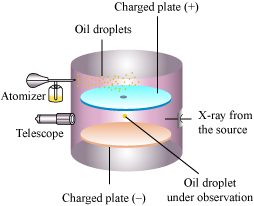
\includegraphics[width = 0.35\textwidth]{1.png}
    \caption{Esquema do arranjo do experimento de Millikan. As gotas eletrizadas de óleo se movem sob a ação de um campo elétrico no interior de um capacitor e são observadas através de um telescópio.}
    \label{fig:esquema}
\end{figure}

Nessas condições, um modelo simples para descrever as forças que atuam numa gota de massa $m$, carga $q$, densidade $\rho_0$ e raio $a$, tanto na subida quanto na descida (conforme esquematiza a figura \ref{fig:forcas}), deve ser conter a força peso, $P = m g = 4 / 3 \pi a^3 \rho_0 g$; a força elétrica, $F_e = q E$; a força de empuxo devido ao ar, $F_{\text{emp}} = 4 / 3 \pi a^3 \rho_{\text{ar}} g$ e a força de resistência viscosa de Stokes, $F_v = - 6 \pi \eta a v$, em que $g$ é a aceleração da gravidade, $E$ é o campo elétrico, $\rho_{\text{ar}}$ é a densidade do ar e $\eta$ é o coeficiente da força viscosa. Assim, tem-se o sistema de equações
\begin{equation}
  \begin{array}{ll}\label{eq:forcas}
      \frac{4}{3} \pi a^3 (\rho_0 - \rho_{\text{ar}}) g - 6 \pi \eta a v + q E & \text{(descida)}\\
      \frac{4}{3} \pi a^3 (\rho_0 - \rho_{\text{ar}}) g + 6 \pi \eta a v - q E & \text{(subida)}
  \end{array}
\end{equation}
do qual é possível obter o raio da gota,
\begin{equation}\label{eq:raio}
	a^2 = \frac{9}{4} \eta \frac{(v_d - v_s)}{g (\rho_0 - \rho_{\text{ar}})}\text{.}
\end{equation}
Por fim, obtém-se a carga contida na gota,
\begin{equation}\label{eq:carga}
	q = \frac{3 \pi \eta a (v_d + v_s)}{E}\text{,}
\end{equation}
em que $v_d$ e $v_s$ são suas velocidades de descida e subida, respectivamente.
\begin{figure}[h]
	\centering
	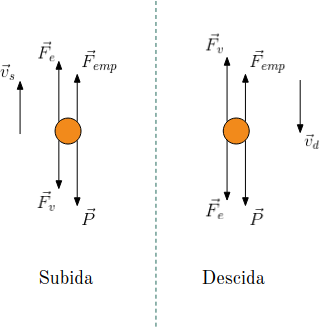
\includegraphics[width = 0.7\linewidth]{forcas-cargas.png}
    \caption{Diagramas de forças atuando numa gota eletrizada nas condições do experimento de Millikan (subida e descida).}
    \label{fig:forcas}
\end{figure}

Todavia, é importante notar que, nas condições do experimento, a força de Stokes necessita de uma correção ao coeficiente de viscosidade que depende da pressão atmosférica e do raio da gota, \cite{apostila}
\begin{equation}\label{eq:etacorr}
	\eta = \frac{\eta_0}{1 + \frac{b}{P a}}\text{.}
\end{equation}

\subsection{Arranjo e procedimento experimental adotado no laboratório didático}

No arranjo adotado no laboratório didático do IFUSP, as gotas de óleo são inseridas entre as placas do capacitor de placas paralelas através de pequenos orifícios na sua placa superior com a ajuda de um atomizador, cujas gotas produzidas têm raios da ordem de \SI{10}{\micro\meter}. O óleo utilizado é um tipo de óleo lubrificante para bombas à vácuo, o qual possui densidade é de \SI{0.8474(9)}{\g\per\cm\cubed} e garante a produção de gotas com cargas positiva e negativa. A tensão entre as placas do capacitor é chaveada manualmente por uma fonte de tensão contínua com amplitude de tensões de \num{0} a \SI{220}{\volt}. Por sua vez, essa tensão é lida através de um multímetro digital do tipo Engro MD-820. As imagens das gotas, iluminadas por uma lâmpada incandescente de \SI{40}{\watt}, são focalizadas em uma das extremidades de um telescópio acoplado ao CCD de uma câmera para computador cujas lentes foram removidas. A estrutura mecânica que suporta o sistema permite que a lâmpada, o capacitor e o telescópio sejam orientados em diversos ângulos, de modo a se evitar a iluminação direta na câmera devido à lâmpada. Gota a gota, as suas trajetórias são obtidas, então, manualmente a partir das imagens capturadas. Para isso, é feita a transformação de medidas em pixels nas imagens para distâncias reais através da calibração com uma escala graduada conhecida.

\begin{figure}[h]
	\centering
    \begin{subfigure}[b]{0.8\linewidth}
    	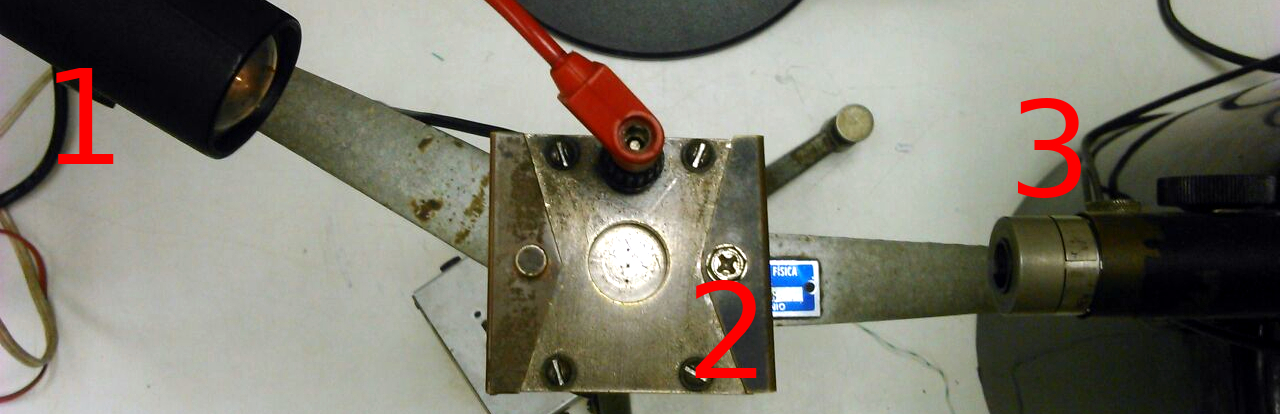
\includegraphics[width = \linewidth]{3.jpeg}
    \end{subfigure}
        \begin{subfigure}[b]{0.8\linewidth}
    	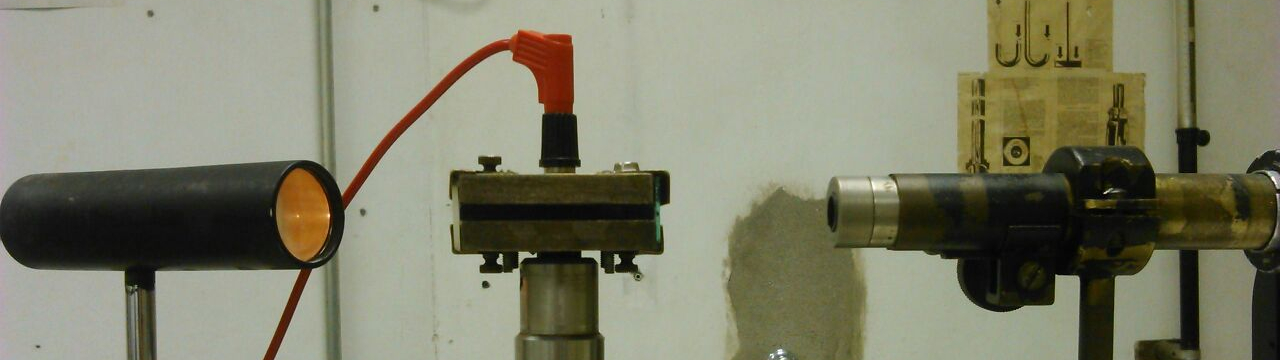
\includegraphics[width = \linewidth]{4.jpeg}
    \end{subfigure}
    \caption{O arranjo opto-mecânico do experimento de Millikan no laboratório didático é composto de uma fonte de luz (1), um capacitor de placas paralelas (2) e um telescópio (3), todos acoplados a um suporte giratório móvel.}
    \label{fig:arranjo}
\end{figure}

Além disso, o laboratório conta com um termômetro e um barômetro para medidas da temperatura e pressão atmosféricas no instante do experimento.

Neste caso, a separação das placas do capacitor foi medida com um paquímetro em \SI{4.50(2)}{\milli\meter}.

% fotos
%% escala de calibração
%% gotejador

\subsection{Dificuldades}

Durante as tentativas de replicar o resultado segundo Millikan utilizando-se o aparato e procedimento adotados no IFUSP, foram notadas diversas dificuldades e obstáculos que dificultam a realização do experimento de modo preciso e rigoroso, dentre as quais se citam:

\begin{itemize}
  \item alto ruído nas imagens capturadas;
  \item baixa resolução espacial e temporal da câmera utilizada;
  \item alta variabilidade da taxa de quadros das imagens adquiridas;
  \item trabalho manual excessivo na análise das trajetórias de cada gota;
  \item baixo contraste devido a iluminação de fundo;
  \item problemas na regulagem e fixação do aparato.
\end{itemize}

Nas turmas anteriores das disciplinas de laboratório em que o experimento foi realizado, notou-se que era necessário um número muito grande de dados (da ordem de 300 gotas) para se obter resultados conclusivos estatísticamente.

O primeiro problema identificado foi a câmera utilizada no arranjo original: ela fornece imagens com uma resolução máxima de \num{640} por \SI{480}{pixels} com uma velocidade de captura nominal de \SI{30}{fps}. Porém, tal velocidade de captura é obtida através de interpolação, com a velocidade real oscilando entre \SI{1}{fps} e \SI{4}{fps}. Sendo assim, os dados obtidos não tinham a qualidade suficiente para uma análise de dados rigorosa, especialmente em um contexto em se deseja automatizar os passos que forem possíveis.

No que tange o arranjo, o maior obstáculo para uma maior precisão nos resultados do experimento é a iluminação. Foi notada uma quantidade de luz de fundo que ofusca consideravelmente as gotas nas imagens obtidas, diminuindo o contraste e a quantidade de gotas selecionadas para análise após cada tomada de dados.

Adicionalmente, verificou-se uma considerável dificuldade em se realizar ajustes finos nas posições dos itens do arranjo, o que dificulta consideravelmente a replicabilidade do experimento - por exemplo, torna-se difícil obter uma boa tomada de dados seguindo-se as recomendações do caderno de instruções adotado.

Em relação à análise dos dados, o método utilizado consistia em obter a trajetória de cada gota manualmente (sem automatização) a fim de se obter as suas velocidades verticais. Isso se mostou excessivamente laboroso levando-se em consideração que o experimento é proposto para estudantes de graduação, ou seja, seria vantajoso que a análise dos dados fosse feita de forma mais rápida.

\section{Aprimoramentos}

\subsection{Aprimoramentos no arranjo}

A primeira ideia a respeito de aprimoramentos do equipamento é acerca da iluminação para que se melhore o contraste entre o fundo e as gotas de óleo.

Foi feita a tentativa de usar os seguintes modos de iluminação:

\begin{itemize}
	\item lâmpada incandescente;
    \item laser vermelho;
    \item LED vermelho.
\end{itemize}

Foi realizada uma adaptação no tubo do telescópio a fim de fixar a câmera para Raspberry Pi.

Adicionalmente, coloca-se a necessidade de existir ajustes mais finos no sistema opto-mecânico para aumentar a replicabilidade e comparabilidade do experimento.

\subsection{Aprimoramentos na aquisição de dados}

Diante dos problemas enumerados na seção anterior, propõe-se a mitigação de diversos deles fazendo-se o uso de um sistema baseado no Raspberry Pi 3 junto com a sua câmera padrão, o qual possui a característica de ser uma plataforma aberta e robusta.

O uso do Raspberri Pi apresenta algumas vantagens em relação ao método anterior. O Raspberry Pi é uma plataforma aberta com performance superior em relação aos computadores disponíveis no laboratório didático do IFUSP, o que se traduz em ganhos de performance que, em tese, possibilitariam a análise das trajetórias das gotas em tempo real. Adicionalmente, a natureza aberta significa que eventuais refinamentos no hardware ou software do arranjo aumentariam a replicabilidade de demais experimentos.

Além disso, a câmera do Raspberry Pi possui uma resolução espaço-temporal superior à anterior: há uma resolução de imagem de \SI{5}{megapixels} e taxas de quadro ajustáveis, podendo variar de \SI{20}{fps} até a ordem de \SI{300}{fps}.

\subsection{Aprimoramentos na análise}

Por último, uma potencialidade na melhora do experimento passa pela automatização da análise de dados usando bibliotecas de código aberto de análise de trajetória como o Trackpy \cite{trackpy}. O uso dessas possibilitaria fazer a análise com muitos mais dados do que se fosse feito manualmente, o que permitiria um maior uso da informação e uma maior precisão dos resultados do experimento. Um exemplo da detecção automática em um quadro está na figura \ref{fig:trackpy}.

\begin{figure}[h]
	\centering
    \begin{subfigure}[b]{0.8\linewidth}
    	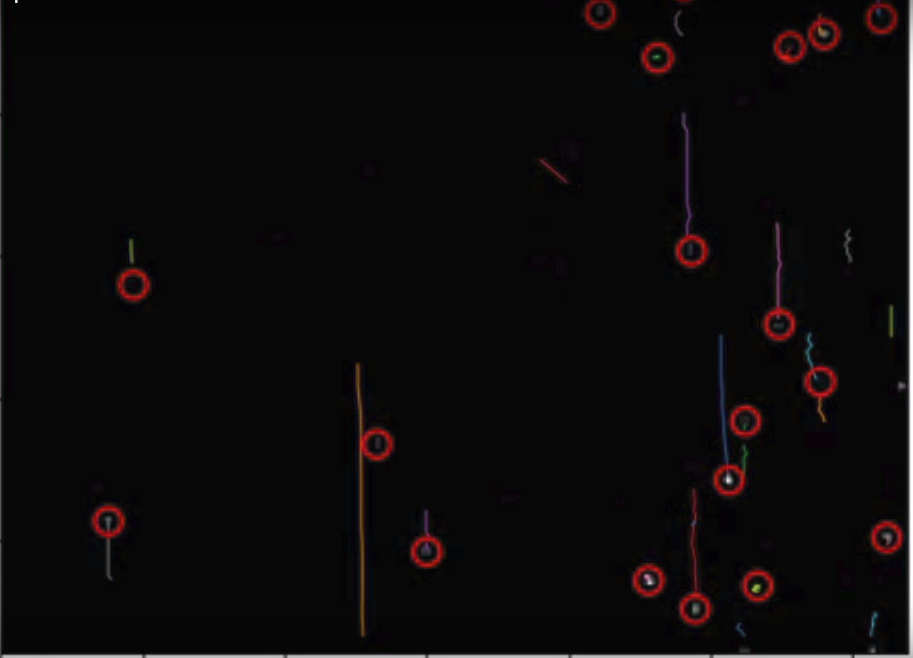
\includegraphics[width = \linewidth]{tracking}
    \end{subfigure}
    \caption{Detecção de gotas e suas trajetórias através da biblioteca Trackpy.}
    \label{fig:trackpy}
\end{figure}

\section{Resultados}

\subsection{Resultados das modificações no arranjo}

No que tange a iluminação, não foi possível visualizar as gotas utilizando-se o laser e o LED vermelhos, e indica-se que uma maior exploração nesse sentido seria necessaria.

\subsection{Resultados das modificações na aquisição de dados}

Ao utilizar o sistema do Raspberry Pi, obteve-se uma melhora sensível na qualidade das imagens adquiridas, especialmente no ruído e na velocidade e consistência da taxa de captura de quadros. A melhora no rúido pode ser vista na figura \ref{fig:cam} enquanto que a consistência pode ser vista na figura \ref{fig:fps}, na qual foi feita uma calibração da taxa de quadros na captura de imagens das gotas. 

\begin{figure}[h]
	\centering
    \begin{subfigure}[b]{0.8\linewidth}
    	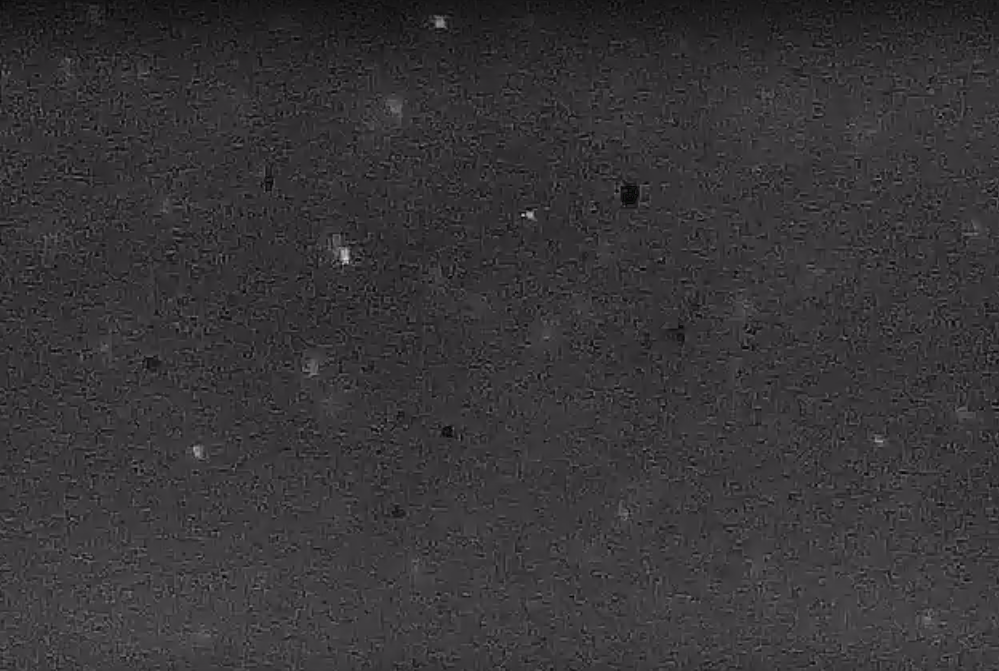
\includegraphics[width = \linewidth]{cam1}
    \end{subfigure}
        \begin{subfigure}[b]{0.8\linewidth}
    	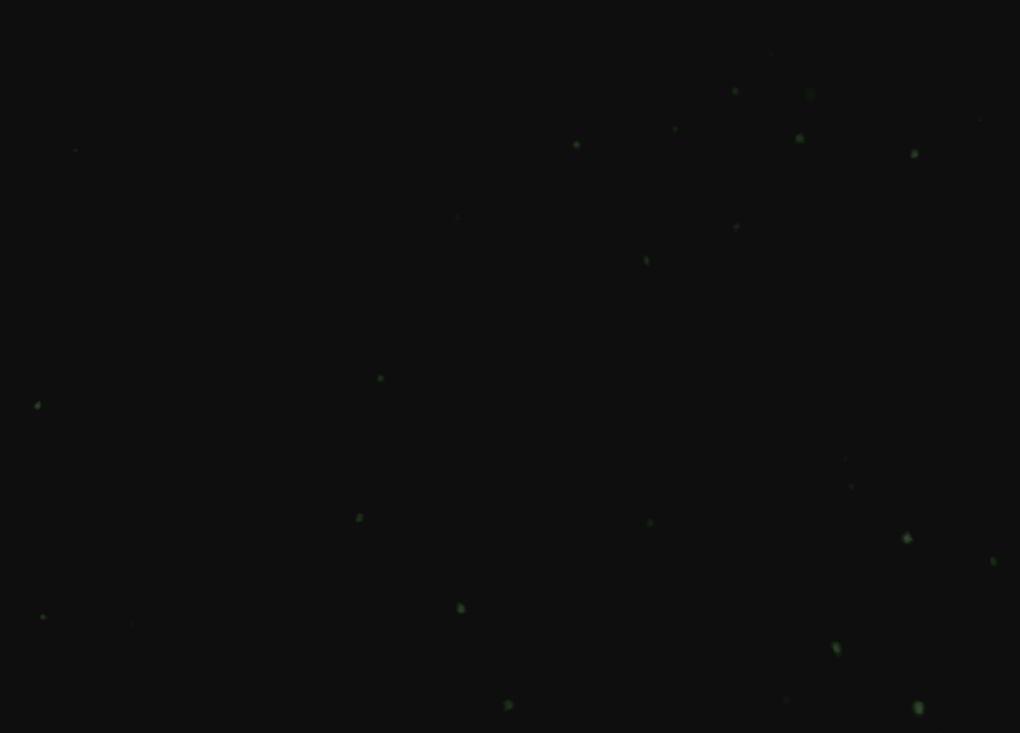
\includegraphics[width = \linewidth]{cam2}
    \end{subfigure}
    \caption{Comparação entre uma imagem da câmera antiga e do Raspberry Pi}
    \label{fig:cam}
\end{figure}

\begin{figure}[h]
	\centering
    \begin{subfigure}[b]{0.8\linewidth}
    	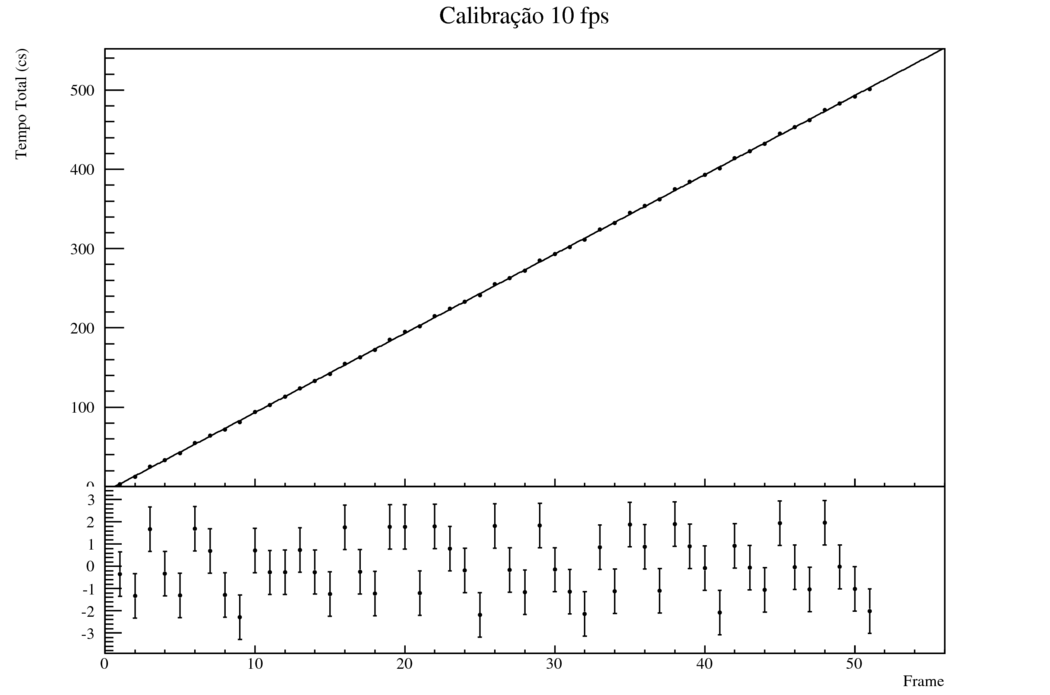
\includegraphics[width = \linewidth]{fps10}
    \end{subfigure}
        \begin{subfigure}[b]{0.8\linewidth}
    	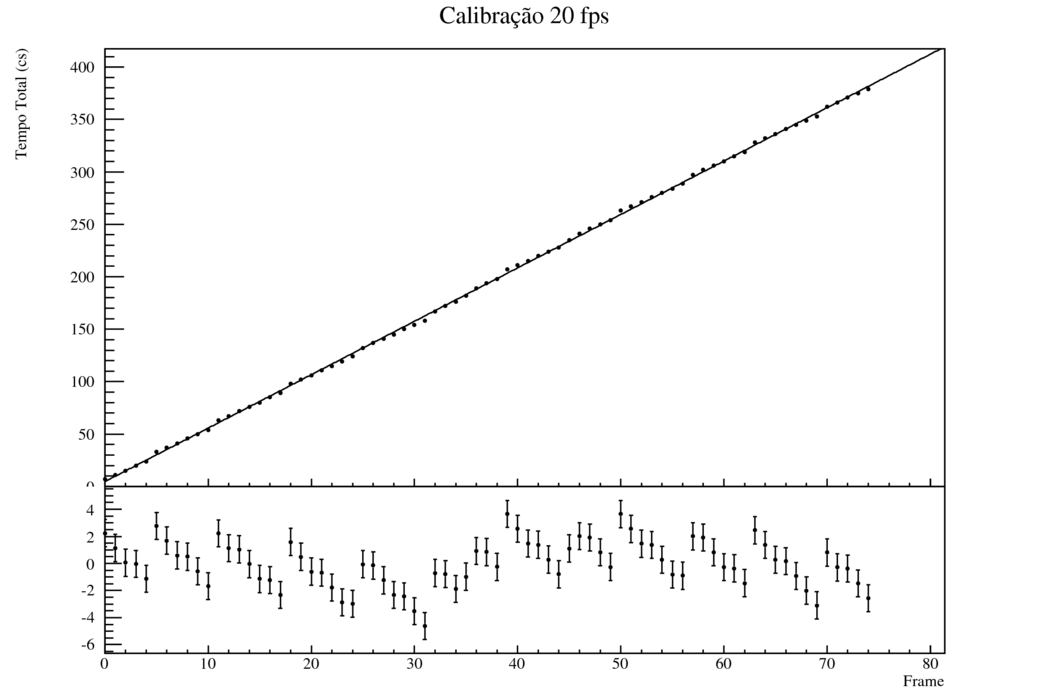
\includegraphics[width = \linewidth]{fps20}
    \end{subfigure}
    \caption{Calibração da taxa de quadros da câmera do Raspberry Pi para 10 e 20 fps, respectivamente. O ajuste da reta aos dados fornece coeficiente angular \SI{9.993(9)}{\centi\second} e \SI{5.091(5)}{\centi\second}, respectivamente, o que é compatível com a taxa nominal de fps.}
    \label{fig:fps}
\end{figure}

\subsection{Resultados da análise de dados}

Para a análise de dados, foi utilizada a biblioteca Trackpy para Python3 para a detecção automática das trajetórias de partículas nos dados adquiridos.

O procedimento adotado foi o seguinte:

\begin{enumerate}
  \item detecta-se as trajetórias das gotas distintas;
  \item divide-se as trajetórias em subtrajetórias utilizando-se a alteração no sentido de velocidade como critério;
  \item obtém-se a velocidade média de cada subtrajetória;
  \item usando a média das velocidades enquanto subindo e enquanto descendo, utiliza-se o procedimento descrito na introdução para obter a carga da gota.
\end{enumerate}

Um exemplo da deteccção de trajetória é dada pela figura \ref{fig:trajetorias}.

\begin{figure}[h]
	\centering
    \begin{subfigure}[b]{0.8\linewidth}
    	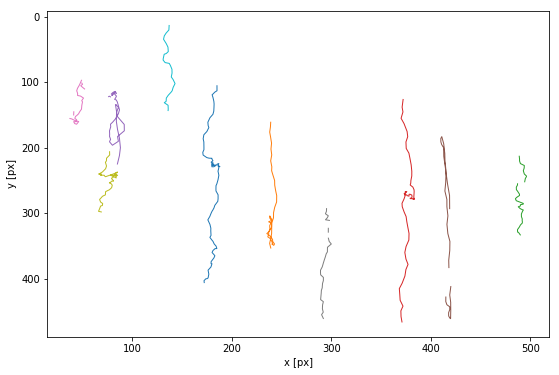
\includegraphics[width = \linewidth]{traj1}
    \end{subfigure}
        \begin{subfigure}[b]{0.8\linewidth}
    	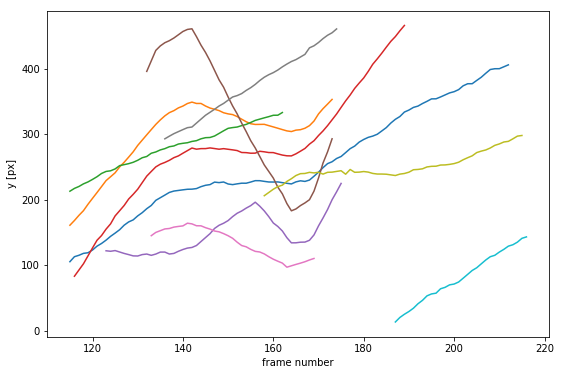
\includegraphics[width = \linewidth]{traj2}
    \end{subfigure}
    \caption{Exemplos da evolução de algumas trajetórias ao longo de 100 frames.}
    \label{fig:trajetorias}
\end{figure}

Adotando então o procedimento acima em uma tomadas de dados, é possível visualizar as cargas obtidas pela figura \ref{fig:resultado}.

\begin{figure}[h]
	\centering
    \begin{subfigure}[b]{0.8\linewidth}
    	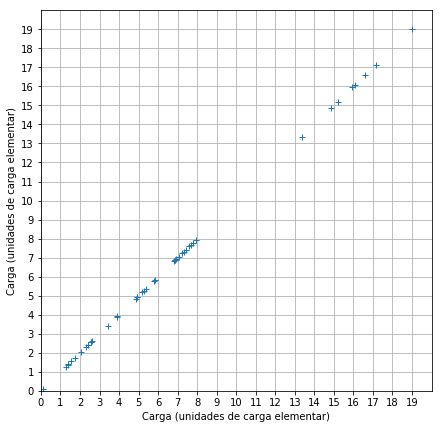
\includegraphics[width = \linewidth]{carga_x_cargas}
    \end{subfigure}
    \caption{Cargas de uma tomada de  dados.}
    \label{fig:resultado}
\end{figure}

\section{Conclusão}

O uso de uma câmera mais robusta junto a análise automatizada de dados se mostraram promissores como aperfeiçoamentos do experimento. Há, porém, a necessidade de se explorar melhor a iluminação do arranjo para que se melhore o contraste das gotas com o fundo -- o qual é o maior fator limitante atual para uma maior precisão do experimento.

\section{Agradecimentos}

Os autores agradecem a Antônio Domingues dos Santos e a Alvimar Floriano de Sousa por todo tipo de suporte neste trabalho.

\section{Referências}

\begin{thebibliography}{99} % Bibliography - this is intentionally simple in this template
\bibitem{millikan} R. A. Millikan. \emph{On the Elementary Electrical Charge and the Avogadro Constant.} 1913.
\bibitem{apostila} IFUSP. \emph{Experimentos de Millikan e movimento browniano.} 2014.
\bibitem{trackpy} D. B. Allan et al. \emph{Trackpy.} Disponível em https://github.com/soft-matter/trackpy. 2014.
\end{thebibliography}

\end{document}
